\documentclass[border=1cm,10pt]{standalone}
\usepackage{tikz}
\usetikzlibrary{arrows}
\usetikzlibrary{decorations.pathmorphing}
\usetikzlibrary{decorations.markings}

\tikzset{
      boson/.style={decorate, decoration={snake}, draw=black, line width=1.2},
      higgs/.style={dashed, draw=red, line width=1.2},
      lepton/.style={draw=blue, line width=1.2, postaction={decorate},
            decoration={markings,mark=at position .55 with {\arrow[draw=blue]{>}}}},
      alepton/.style={draw=blue, line width=1.2,  postaction={decorate},
            decoration={markings,mark=at position .55 with {\arrow[draw=blue]{<}}}},
      quark/.style={draw=blue, line width=1.2,  postaction={decorate},
            decoration={markings,mark=at position .55 with {\arrow[draw=blue]{>}}}},
      aquark/.style={draw=blue, line width=1.2,  postaction={decorate},
            decoration={markings,mark=at position .55 with {\arrow[draw=blue]{<}}}},
}


\begin{document}

    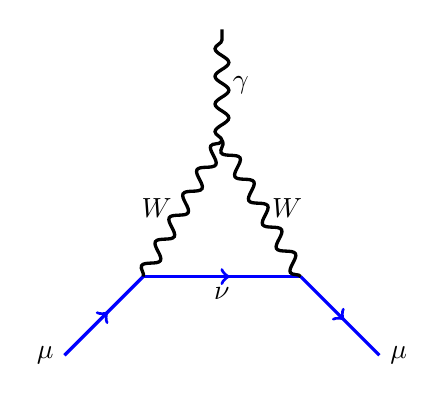
\begin{tikzpicture}

        \draw[lepton] (0,0) node[left] {$\mu$} -- (1,1) ;
        \draw[lepton] (3,1) -- (4,0) node[right] {$\mu$} ;
        \draw[lepton] (1,1) -- (3,1) node[midway,below] {$\nu$} ;

        \draw[boson] (1,1) -- (2,2.73) node[midway,left] {$W$} ;
        \draw[boson] (3,1) -- (2,2.73) node[midway,right] {$W$} ;

        \draw[boson] (2,2.73) -- (2,4.14) node[midway,right] {$\gamma$} ;

    \end{tikzpicture}

\end{document} 
